%% ==============================
\chapter{State of the art}
\label{sec:state_of_the_art}
%% ==============================
Questions to ask:
\begin{enumerate}
    \item What is generally known about the topic? (relevant theory)
    \item What are the most important (recent) existing works in the field related to the research problem? 
    \item Provide a comprehensive review of the relevant literature, including key theories, concepts, and previous studies that inform your research question.
    \item What are the limitations or gaps in the existing works that this work aims to address? 
    \item How does this work build upon or differ from existing works? 
    \item What are the main research approaches or techniques used in the field, and how do they relate to this work? 
    \item What are the main challenges or open questions in the field? 
\end{enumerate}

General theory:
\begin{enumerate}
    \item Path planning
    \item Astar, RRT, Dijkstra, PRM
    \item Hierarchical graphs
    \item ROS2 Nav Stack
    \item OpenRMF
    \item Behavior Trees
\end{enumerate}

Other approaches to Q1 (Navigate in large multi-story environments):
\begin{enumerate}
    \item Paper IAS-17 Autonomous Hierachy Creation for Path Planning of Mobile Robots in Large Environments
    \item Paper Hierarchical Path-Planning for Mobile Robots Using a Skeletonization-Informed Rapidly Exploring Random Tree*
\end{enumerate}

Other approaches to Q2 (Plan paths that are straight, deterministic and human-predictable):
\begin{enumerate}
    \item Voronoi Diagrams, EVG (with sensory horizont)
    \item Smoothing algorithms (Bezier curves, B-Splines, Bechtold and Glavina, Latombe)
    \item Paper Straight Skeleton Based Automatic Generation of Hierarchical Topological Map in Indoor Environment
\end{enumerate}

Research gap from previous approaches:
\begin{enumerate}
    \item Hierarchical graphs are not per room or per floor which makes it difficult to append slamed maps or semantic information
    \item Hierarchical graphs are not used in ROS2 Nav Stack
    \item Approaches for straight paths are not deterministic and not human-predictable
    \item Approaches for straight paths are not implemented in ROS2 Nav Stack
    \item Approaches for straight paths only work well in small corridors
\end{enumerate}

The following overview of the state of the art consits of four main parts. First, the general theory of path planning in mobile robotics is presented. This includes the most common algorithms for path planning, and their applications in real robotic systems. Second, the recent approaches to hierarchical planning in large multi-story environments are presented. This shows the existing approaches to the first research question: "How to navigate in large multi-story environments?" Third, the recent approaches to straight paths and smoothing are presented. This shows the existing approaches to the second research question: "How to plan paths that are straight, deterministic and human-predictable?" Finally, in chapter \ref*{sec:research_gap} the research gap and limitations of the state of the art is summarized.

%% ==============================
\section{General Path Planning for Mobile Robots}
\label{sec:path_planning}
%% ==============================

The general approach to path planning in mobile robotics is a two-layered architecture which can be seen in Figure \ref{XX} \todo{Quelle probabalistic robotics and graphic from ppt} The first layer is the global path planning layer. It is responsible for finding a path from the start to the goal position in a previously known static environment. The second layer is the collision avoidance also known as local path planner or controller. It is responsible for avoiding dynamic obstacles that prevent the global path from being executed. For both layers there are different approaches as open source solutions available. The scope of this work is limited to extending the capabilities of the global planner for multiple floors. The collison avoidance is solved with existing algorithms. The following sections will give an overview of the most common planner algorithms. 

%% ==============================
\subsection{Path Planning Algorithms}
Planning a path is a major challenge in robotics and is necessary for mobility. The path from the robot's current location to the goal can be planned in two ways: deterministically or probabilistically. Deterministic planners use algorithms that always deliver the same results with the same input. Probabilistic planners, on the other hand, are based on randomness and produce different results for the same input. The map on which deterministic planners are based is usually discretised into a lattice. In an informed search, heuristics can be used to tell whether one grid field is closer to the target configuration than another. According to Burgard in \cite{XXBurgard}, the performance of a search algorithm is measured in four different ways:
\begin{enumerate}
    \item Completeness:
    Does the algorithm find the solution if there is one?
    \item Optimality:
    Is the solution the best of all possible solutions in terms of path cost?
    \item Time complexity:
    How long does it take to find a solution?
    \item Space complexity:
    How much memory is needed to perform the search?
\end{enumerate}

%% ==============================
\subsection{The Robot Operating System 2}
\begin{displayquote}
    \enquote{The \acrfull{ros} is a framework for writing robot software. It is a collection of tools, libraries, and conventions that aim to simplify the task of creating
    complex and robust robot behavior across a wide variety of robotic platforms.} \cite{Quigley.2015}
\end{displayquote}
    
\begin{figure}[h]
    \centering
    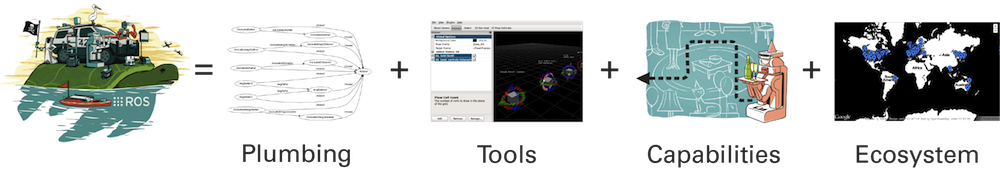
\includegraphics[width=1\textwidth]{figures/02_state_of_the_art/ros_equation.png}
    \caption{The ROS equation: ROS = Plumbing + Tools + Capabilities + Community (Source: \cite{OpenRobotics_About.2020})}
    \label{fig:ros_equation}
\end{figure}

The development of \gls{ros} began in 2007 as part of the Stanford AI Robot Project (STAIR) and was mainly driven by Willow Garage. There it was used as the basis for the Personal Robot 2 (PR2), but has been intended from the start as an open-source platform for a wide range of robotic applications. By now, the development is being driven forward by Open Robotics. The founders, Brian Gerkey and Morgan Quigley, have also published a comprehensive book to make it easier to get started with ROS \cite{Quigleyetal}. The ROS ecosystem consists of much more than pure code; it thrives on a large community and the exchange of ready-to-use packages, which is described by the 'ROS equation' in Figure \ref{fig:ros_equation}. Since 2011, ROS has has left the earth for the International Space Station with NASA's Robonaut 2 \cite{Diftleretal.2011}, \cite{Badgeretal.2016}. Due to the rapidly growing community and increasing application in industry, an improved version was developed and released in December 2018 as ROS 2. The main difference is the focus on real-time applications and the use of the industry standard 'Data Distribution Service' (DDS) for the communication of distributed systems.

Nodes are the basis of the distributed network of an ROS application. The nodes are executed independently of each other and communicate with each other via defined interfaces. This offers the advantage that applications can be built up modularly, can be easily exchanged, and can be used in conjunction with other applications. A node can contain several topics, services or actions with which data can be exchanged with other nodes. Different nodes in a ROS application can be executed on different hardware. A collection of nodes that perform a completed function are grouped together as a package and shared by many developers around the world. A combination of related packages with a version history and managed documentation is called a stack. For example, there is the Navigation Stack, which contains all the functions needed to move the robot safely from A to B. This includes algorithms for localisation and path planning as well as the processing of sensor data for obstacle avoidance and mapping.

\begin{figure}[h]
    \centering
    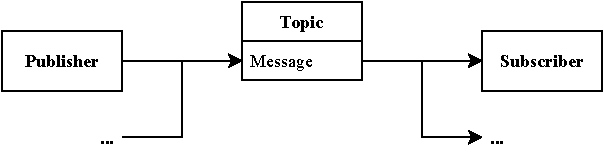
\includegraphics[width=0.75\textwidth]{figures/02_state_of_the_art/topics.pdf}
    \caption{The structure of a topic}
    \label{fig:topics}
\end{figure}

The individual nodes communicate through message channels about a specific topic. This communication is designed for distributed systems and enables a many-to-many (n:m) cardinality. This means that each node can act as a publisher or subscriber of any topic, see Figure \ref{fig:topics}. The content of the message is defined by a .msg file as the interface.

\begin{figure}[h]
    \centering
    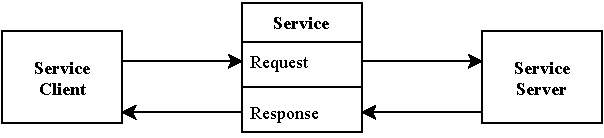
\includegraphics[width=0.75\textwidth]{figures/02_state_of_the_art/services.pdf}
    \caption{The structure of a service}
    \label{fig:services}
\end{figure}

Services are based on the call-and-response model. This means that, unlike topics, messages are not unilaterally sent into the network. Instead, a request is made from a client to a server, and a response is sent back, as illustrated in Figure \ref{fig:services}. The structure resembles a function call, where parameters are passed and a return value is expected. The data types are defined in the corresponding .srv file. This type of communication is particularly useful for computations performed by another node \cite(Quigleyetal.,2015,p.51). Services can be executed synchronously or asynchronously. In a synchronous call, the calling node blocks the thread until the response arrives. Synchronous calls should only be used when the service requires a short, finite amount of time for computation. Asynchronous calls are implemented by providing a predefined function (callback) that is automatically invoked by ROS when the service response is received. This allows other code to be executed in the node as long as it does not depend on the service result.

\begin{figure}[h]
    \centering
    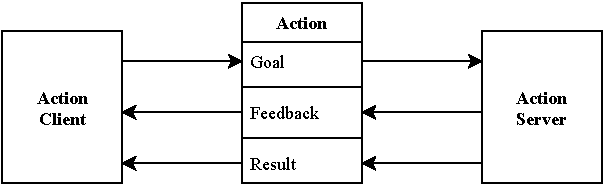
\includegraphics[width=0.75\textwidth]{figures/02_state_of_the_art/actions.pdf}
    \caption{The structure of an action}
    \label{fig:actions}
\end{figure}

Actions have been a fixed component of the communication vocabulary since ROS 2. They are designed for the asynchronous execution of long-duration actions. In addition to the concept of services, actions allow for the exchange of feedback data during execution. Furthermore, actions provide the ability to cancel their execution. An action client sends a request (goal) to the action server, which can either accept or reject the goal. During execution, a feedback callback is invoked at the client until the result is received and processed. Actions offer a high-level communication protocol, as shown in Figure \ref{fig:actions}. A good example of the application of actions is robot movement towards a specific goal. The task should occur asynchronously and can vary in duration. Through the feedback mechanism, information about the current position of the robot can be communicated, and if the goal becomes outdated, the action can be canceled. The interface of an action for navigation is defined by an .action file, as depicted in Algorithm \ref{lst:navigatetopose.action}.

\lstset{language=python, caption={NavigateToPose.action, definition of an action from type 'NavigateToPose'}, label={lst:navigatetopose.action}}
\begin{lstlisting}
# goal
geometry_msgs/PoseStamped pose
-%{}%-%{}%-
# result
std_msgs/Empty result
-%{}%-%{}%-
# feedback
geometry_msgs/PoseStamped current_pose
builtin_interfaces/Duration navigation_time
int16 number_of_recoveries
float32 distance_remaining
\end{lstlisting}
    
%% ==============================
\subsubsection{The Navigation Stack in ROS2}

\begin{displayquote}
    \enquote{Nav2 is the professionally supported spiritual successor of the ROS Navigation Stack. This project seeks to find a safe way to have a mobile robot move to complete complex tasks through many types of environments and classes of robot kinematics. Not only can it move from Point A to Point B, but it can have intermediary poses, and represent other types of tasks like object following and more. Nav2 is a production-grade and high-quality navigation framework trusted by 50+ companies worldwide.} \cite{https://navigation.ros.org/}
\end{displayquote}

The Navigation2 stack for \gls{ros_2} is a comprehensive framework for the development of new planner algorithms. The planner developed in this work is based on the Nav2 stack and is written as an exchangable plugin for the existing structure. With its server and plugin layout Nav2 supports custom planner, controller behavior and smoother plugins. In Figure \ref{fig:nav2_architecture} the architecture of Nav2 is shown. It follows the classic two-layered architecture for path planning seen in Figure \ref{XX}. The planner server provides the global path planning on a known map and the controller server offers algorithms for follwoing this path with dynamic obstacle avoidance. The necessary inputs for this system are the map, the odometry of the robot wheels and the sensor data from lidars or cameras. With these informations the localization can calculate the most likely position of the robot in the map. The planner plans a path from this current position to the goal. In a control loop, the controller tries to reduce the error between the current position and the planned path. The output of the controller is a velocity command for the robot. The velocity command is then executed by the robot's motor controller.

\begin{figure}[h]
    \centering
    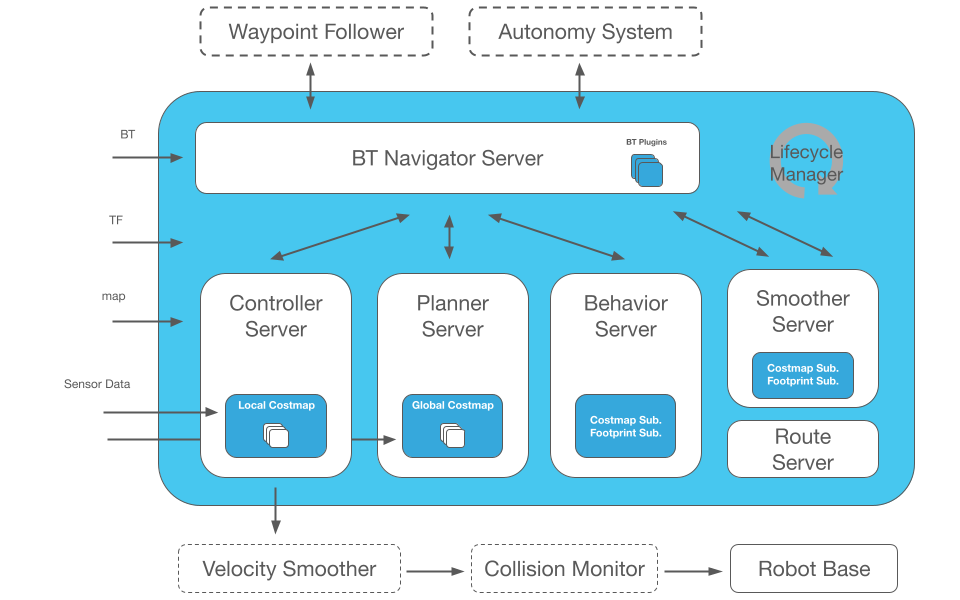
\includegraphics[width=\textwidth]{figures/02_state_of_the_art/nav2_architecture.png}
    \caption{The architecture of the Nav2 stack (Source: \cite{https://navigation.ros.org/})}
    \label{fig:nav2_architecture}
\end{figure}

In this work a new planner, capable of planning in complex multi-story environments, is developed. The algorithm is implemented as a plugin for the planner server. The rest of the Nav2 pipeline is used with existing packages.

%% ==============================
\subsubsection{Behavior Trees for Navigation}

Nav2 is the most prominent example of \glspl{bt} in robotics and especially for navigation. It uses \glspl{bt} to create customized and intelligent navigation behavior by orchestrating many independent modular servers. The default \gls{bt} for executing a navigation request to a specific goal is shown in Figure \ref{fig:nav_bt}. It shows the actual planner, an A* algorithm, on the left side which is triggered every second (1 Hz). All other named actions are recovery behaviors which are used to clear the costmaps and reorient the robot if it gets stuck. To understand the symbolic language of the \gls{bt} the single elemnts are explained in the following section.

\begin{figure}[h]
    \centering
    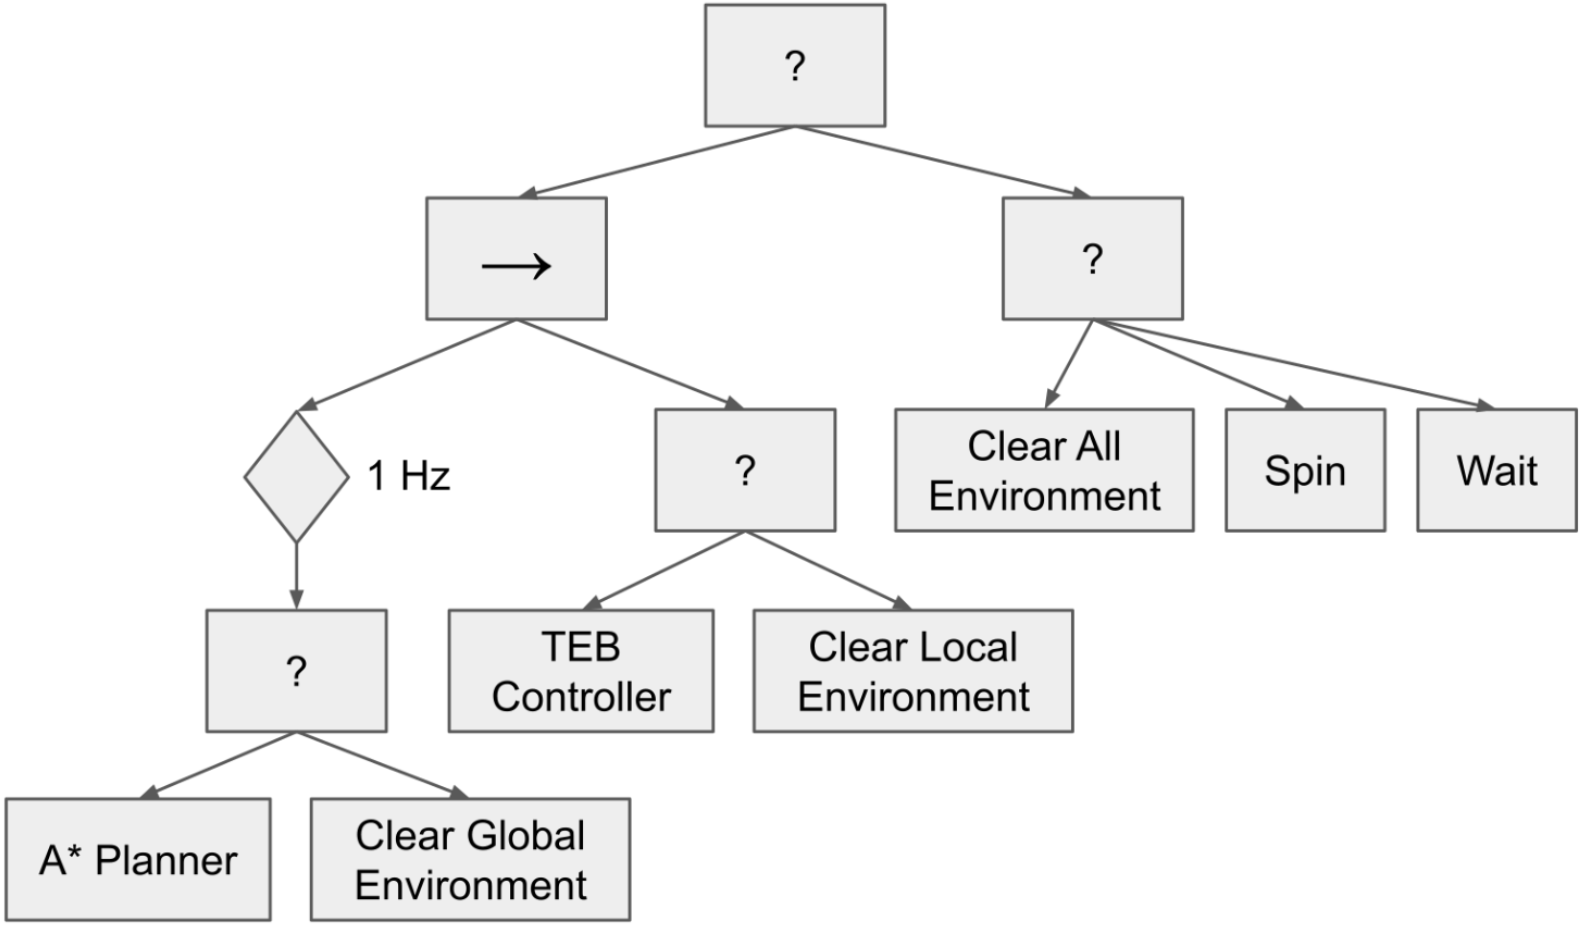
\includegraphics[width=\textwidth]{figures/02_state_of_the_art/nav2_bt.png}
    \caption{The default navigation behavior (Source: \cite{Marathon})}
    \label{fig:nav2_bt}
\end{figure}

\Glspl{bt} were developed for video games to describe the behavior of computer-controlled characters in a modular way \cite{Limetal.,2010}. BTs combine a deliberative approach with reactive components. The internal structure of the tree establishes an overall plan of actions, ensuring goal-oriented behavior. However, reactive behavior can still be triggered through constant reevaluation of all conditions. 

A \gls{bt} consists of small building blocks that can be combined to create any control structure. The biggest difference from State Machines is that in \glspl{fsm}, a state-dependent transition is triggered after a specific input. In \glspl{bt}, on the other hand, the entire structure is updated at regular, short time intervals, and all conditions are re-evaluated. This allows for arbitrary transitions to occur based on the appropriate preconditions, without explicitly defining them.

The fundamental element of every \gls{bt} is the root node, from which the attached nodes are updated (ticked). Each node returns either Success, Failure, or Running after being updated. In general, a \gls{bt} can be described using an \gls{fsm}, where the state transitions can take three possible states into account, as shown in Figure \ref{fig:fsm_general_bt}.

\begin{figure}[h]
    \centering
    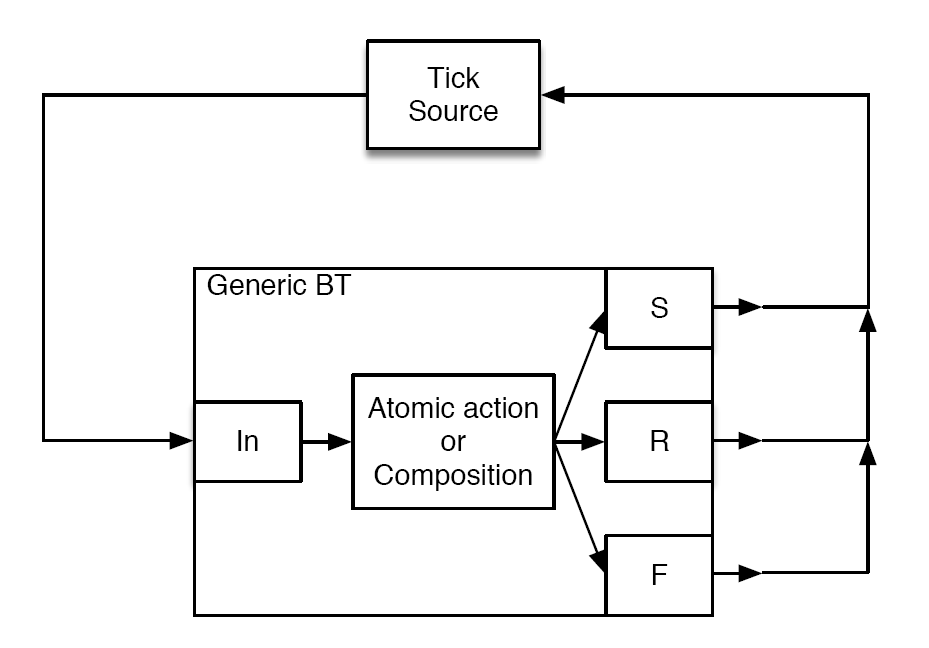
\includegraphics[width=0.7\textwidth]{figures/02_state_of_the_art/fsm_general_bt.png}
    \caption[Allgemeiner \textit{Behavior Tree} als FSM]{Darstellung eines allgemeinen \gls{bt} durch eine \gls{fsm} mit den Zustandsübergängen \textit{Success} (S), \textit{Running} (R) und \textit{Failure} (F) (Source: Colledanchise.2018)}
    \label{fig:fsm_general_bt}
                          \end{figure}

The basic building blocks of a BT are shown in Figure \ref{fig:bt_types}. Actions represent individual, self-contained algorithms that execute specific commands to actuators or perform calculations. An Action can run in a blocking (synchronous) manner, where it returns either Success or Failure after its start, or it can run asynchronously and maintain a Running state during execution. Conditions, on the other hand, take either Success or Failure states depending on the condition being evaluated.

\begin{figure}[h]
    \centering
    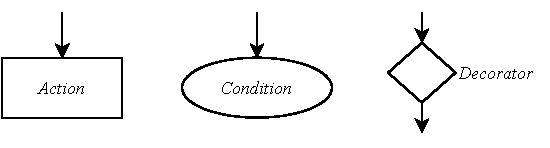
\includegraphics[width=0.7\textwidth]{figures/02_state_of_the_art/bt_types.pdf}
    \caption{Graphische Darstellung von \textit{Actions}, \textit{Conditions} und \textit{Decorators}}
    \label{fig:bt_types}
\end{figure}

The Decorator is a type of control node that has only one child. It allows the state of the child node to be influenced by custom-defined rules, avoiding complex constructions with Sequences and Fallbacks. Examples of Decorators include Inverters, Time Delays, and Repeaters (repeating a certain number of times or until a successful completion).

\begin{figure}[h]
    \centering
    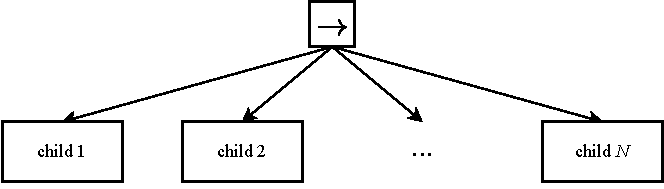
\includegraphics[width=0.75\textwidth]{figures/02_state_of_the_art/sequence.pdf}
    \caption{Graphical BT of a Sequence with \textit{N} childs}
    \label{fig:sequence}
\end{figure}

\lstset{language=C++, caption={Algorithm of a Sequence with \textit{N} childs}, label={lst:pseudo_code_sequence}, morekeywords={from, to}}
\begin{lstlisting}[float=h]
for i from 1 to %\textit{N}% do
    child_status = tick(child[i])
    
    if child_status == %\textit{Running}%
        return %\textit{Running}%
        
    if child_status == %\textit{Failure}%
        return %\textit{Failure}%

return %\textit{Success}%
\end{lstlisting}

The Sequence starts its children from left to right in the graphical representation, as shown in Figure \ref{fig:sequence}. If a child returns Running, the entire Sequence is considered Running. Upon successful execution of a child, the next child is started, continuing until all children, and thus the entire Sequence, achieve the Success state. If a child cannot be executed successfully, the loop is aborted, and the Sequence enters the Failure state, as shown in Algorithm \ref{lst:pseudo_code_sequence}.
  

\begin{figure}[h]
    \centering
    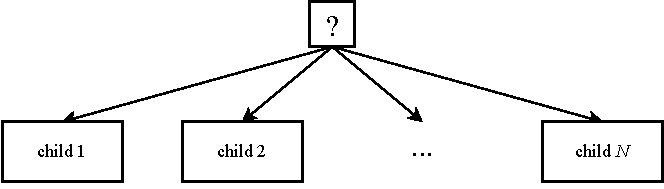
\includegraphics[width=0.75\textwidth]{figures/02_state_of_the_art/fallback.pdf}
    \caption{Graphical BT of a Fallback with \textit{N} childs}
    \label{fig:fallback}
  \end{figure}
  
  \lstset{language=C++, caption={Algorithm of a Fallback with \textit{N} childs}, label={lst:pseudo_code_fallback}, morekeywords={from, to}}
  \begin{lstlisting}[float=h]
  for i from 1 to %\textit{N}% do
      child_status = tick(child[i])
      
      if child_status == %\textit{Running}%
          return %\textit{Running}%
          
      if child_status == %\textit{Success}%
          return %\textit{Success}%
  
  return %\textit{Failure}%
  \end{lstlisting}

  A Fallback node (also known as Selector) executes only one child successfully, unlike the Sequence. All children are updated from left to right, as shown in Figure \ref{fig:fallback} and Algorithm \ref{lst:pseudo_code_fallback}. Once a child reaches the Success state, the Fallback is completed. If a child returns Failure, the next child is started.

\begin{figure}[h]
    \centering
    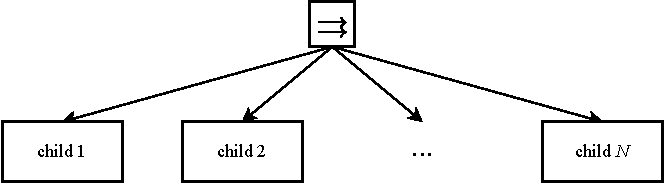
\includegraphics[width=0.75\textwidth]{figures/02_state_of_the_art/parallel.pdf}
    \caption{Graphical BT of a Parallel with \textit{N} childs}
    \label{fig:parallel}
\end{figure}
  
\lstset{language=C++, caption={Algorithm of a Parallel with \textit{N} childs and success count \textit{M}}, label={lst:pseudo_code_parallel}, morekeywords={from, to}}
\begin{lstlisting}[float=h]
for i from 1 to %\textit{N}% do
    child_status[i] = tick(child[i])
    
if success_count(child_status) >= %\textit{M}%
    return %\textit{Success}%
        
if failure_count(child_status) > (%\textit{N}% - %\textit{M}%)
    return %\textit{Failure}%

return %\textit{Running}%
\end{lstlisting}

In addition to the control nodes Sequence and Fallback, there is also the Parallel node. In this structure, all children are started simultaneously, and the final state of the Parallel node is determined based on a comparison between a defined count M and the number of successfully completed children, as shown in Figure \ref{fig:parallel} and Algorithm \ref{lst:pseudo_code_parallel}.

An overview of the functions of each element is presented in Table \ref{tab:overview_bt}.

\begin{table}[h]
\centering
\resizebox{\textwidth}{!}{%
%\setlength{\extrarowheight}{8pt}
\begin{tabular}{lclll}
\toprule
\textbf{} & \multicolumn{1}{l}{\textbf{}} & \multicolumn{3}{c}{\textbf{Return Status}} \\ \midrule
\multicolumn{1}{c}{\textbf{Type}} & \textbf{Symbol} & \multicolumn{1}{c}{\textbf{Success}} & \multicolumn{1}{c}{\textbf{Failure}} & \multicolumn{1}{c}{\textbf{Running}} \\ \midrule
\textbf{Action} & Text & When completed & In case of errors & During execution \vspace{3mm}\\
\textbf{Condition} & Text & When condition is true & When condition is false & Never \vspace{3mm}\\
\textbf{Sequence} & $\to$ & When all children are \textit{Success} & When a child is \textit{Failure} & When a child is \textit{Running} \vspace{3mm}\\
\textbf{Fallback} & ? & When a child is \textit{Success} & When all children are \textit{Failure} & When a child is \textit{Running} \vspace{3mm}\\
\textbf{Parallel} & $\rightrightarrows$ & \begin{tabular}[c]{@{}l@{}}When $\ge$ \textit{M} \\ children are \textit{Success}\end{tabular} & \begin{tabular}[c]{@{}l@{}}When > \textit{N} - \textit{M} \\ children are \textit{Failure}\end{tabular} & \begin{tabular}[c]{@{}l@{}}As long as limits \\ are not reached\end{tabular} \vspace{3mm}\\
\textbf{Decorator} & $\diamond$ & Depending on the function & Depending on the function & Depending on the function \\ \bottomrule
\end{tabular}%
}
\caption{Overview of the elements of a Behavior Tree}
\label{tab:overview_bt}
\end{table}

BTs represent an evolution of \gls{fsm}, which are still widely used, but offer several advantages beyond them. The following are the advantages and drawbacks of \glspl{bt}. These characteristics are not necessarily unique to \glspl{bt} but also apply to other concepts such as \glspl{hfsm} or decision trees \cite{ColledanchiseandÖgren,2018,pp.37ff.}.

\begin{enumerate}
  \item \textbf{Modularity:} Individual subsystems can be modified and replaced as needed. The entire BT can also be reused as a module.
  \item \textbf{Hierarchical Structure:} Each control node introduces an additional level of hierarchy, making the overall behavior easier to understand.
  \item \textbf{Reusability:} Defined interfaces allow code to be used in multiple locations.
  \item \textbf{Reactiveness:} By continuously updating the BT, actions can be executed in a closed loop, enabling dynamic responses to the environment.
  \item \textbf{Intuitive Representation:} The graphical representation remains understandable even for complex systems.
  \item \textbf{Automatic Analysis:} Tools exist to monitor robustness and efficiency. BTs can also be created and monitored live using graphical editors.
  \item \textbf{Automatic Generation:} BTs can be generated during execution using machine learning techniques.
\end{enumerate}

However, there are also some disadvantages of BTs:

\begin{enumerate}
  \item \textbf{Complexity of the Engine:} Ensuring parallelism is necessary, but there are existing frameworks available to handle this.
  \item \textbf{Computational Intensity:} Updating all control nodes and conditions at each tick can be computationally intensive, potentially affecting real-time performance on weaker systems.
  \item \textbf{Implementation Overhead for Simple Behaviors:} For very short behaviors, direct programming or a simple FSM may be more efficient.
  \item \textbf{Immaturity of Behavior Trees:} Compared to widely adopted FSMs, there are fewer applications and software available for BTs.
\end{enumerate}


%% ==============================
\section{Hierarchical Planning for Multi-Story Environments}
\label{sec:hierarchical_planning}
%% ==============================

%% ==============================
\section{Straight Paths and Smoothing}
\label{sec:straight_paths}
%% ==============================

%% ==============================
\section{Research Gap and Limitations}
\label{sec:research_gap}
%% ==============================
